\documentclass{article}
\usepackage{arxiv}

\usepackage[utf8]{inputenc}
\usepackage[english, russian]{babel}
\usepackage[T1]{fontenc}
\usepackage{url}
\usepackage{booktabs}
\usepackage{amsfonts}
\usepackage{nicefrac}
\usepackage{microtype}
\usepackage{lipsum}
\usepackage{graphicx}
\usepackage{natbib}
\usepackage{doi}



\title{Автоматический подбор гиперпараметров моделей машинного обучения}

\author{ Надршена Вероника Рафиковна  \\
	МГУ им. М.В. Ломоносова\\
	ф-т ВМК, кафедра ММП\\
	% Pittsburgh, PA 15213 \\
	\texttt{s02190794@gse.cs.msu.ru} \\
	%% examples of more authors
	\And
	д.ф-м.н. Китов Виктор Владимирович\\
	МГУ им. М.В. Ломоносова\\
	ф-т ВМК, кафедра ММП\\
	% Santa Narimana, Levand \\
	%% \AND
	%% Coauthor \\
	%% Affiliation \\
	%% Address \\
	%% \texttt{email} \\
	%% \And
	%% Coauthor \\
	%% Affiliation \\
	%% Address \\
	%% \texttt{email} \\
	%% \And
	%% Coauthor \\
	%% Affiliation \\
	%% Address \\
	%% \texttt{email} \\
}
\date{}

\renewcommand{\shorttitle}{\textit{arXiv} Template}

%%% Add PDF metadata to help others organize their library
%%% Once the PDF is generated, you can check the metadata with
%%% $ pdfinfo template.pdf
\hypersetup{
pdftitle={Методы верификации для кластеризации временных рядов},
pdfsubject={q-bio.NC, q-bio.QM},
pdfauthor={David S.~Hippocampus, Elias D.~Striatum},
pdfkeywords={First keyword, Second keyword, More},
}

\begin{document}
\maketitle

\begin{abstract}
	В данной работе рассматривается задача автоматического подбора гиперпараметров для моделей машинного обучения. Традиционные методы ручного выбора или простого перебора гиперпараметров (Grid Search) часто оказываются трудоемкими и не всегда приводят к наилучшим результатам. В связи с этим возникает необходимость в исследовании и применении более продвинутых методов автоматической оптимизации гиперпараметров.

    Целью работы является изучение, анализ и сравнение современных методов автоматического подбора гиперпараметров, таких как Random Search, байесовская оптимизация и эволюционные алгоритмы, и определение их применимости и эффективности в различных задачах машинного обучения.
\end{abstract}


\keywords{Grid Search \and Random Search \and байeсовская оптимизация}

\section{Введение}
В области машинного обучения процесс создания оптимальной модели часто включает в себя настройку гиперпараметров, что является критически важным этапом для достижения высокой производительности алгоритма. Гиперпараметры, в отличие от параметров модели, не обучаются непосредственно в процессе обучения, но они могут существенно влиять на качество итоговой модели. Например, коэффициент обучения, количество скрытых слоев в нейронной сети или параметры регуляризации — это лишь некоторые из гиперпараметров, которые нужно правильно выбрать.

Традиционные методы настройки гиперпараметров, такие как ручной подбор или сеточный поиск, могут быть трудоемкими и неэффективными, особенно при наличии большого числа гиперпараметров или при необходимости оптимизации сложных моделей \citep{bergstra2012}. В связи с этим автоматический подбор гиперпараметров становится все более популярным, так как он предлагает методы, способные автоматически и эффективно исследовать пространство гиперпараметров и находить оптимальные комбинации.

Алгоритмы автоматического подбора гиперпараметров, такие как байесовская оптимизация, генетические алгоритмы или градиентный подбор, показали свою эффективность в ряде исследований \citep{snoek2012, thornton2013}. Благодаря этому они стали неотъемлемой частью современных систем машинного обучения.

Однако, несмотря на прогресс в этой области, существует множество открытых вопросов и проблем. Основные трудности заключаются в масштабируемости алгоритмов, выборе подходящего метода для конкретной задачи или проблемах связанных со стабильностью и интерпретируемостью результатов.

В целом, автоматический подбор гиперпараметров продолжает оставаться актуальной и важной областью исследований в мире машинного обучения, и многие исследователи и практики постоянно ищут новые и улучшенные методы решения этой задачи.

\section{Постановка задачи}
Рассмотрим множество моделей машинного обучения \( \mathcal{M} \). Для каждой модели \( m \in \mathcal{M} \) определим пространство гиперпараметров как \( \mathcal{H}_m \). Пусть \( L: \mathcal{M} \times \mathcal{H}_m \rightarrow \mathbb{R} \) представляет функцию потерь, которая оценивает качество соответствующей модели на заданном наборе данных при определенной комбинации гиперпараметров.

Задача автоматического подбора гиперпараметров может быть сформулирована следующим образом:

\[
(m^*, h^*) = \arg\min_{m \in \mathcal{M}, h_m \in \mathcal{H}_m} L(m, h_m).
\]

Цель состоит в том, чтобы найти такие \( m^* \) и \( h^* \), при которых функция потерь достигает минимального значения. Традиционные методы, такие как сеточный поиск, могут быть неэффективными в ситуациях с большим пространством гиперпараметров~\citep{bergstra2012}. С другой стороны, более современные методы, такие как байесовская оптимизация или эволюционные алгоритмы, предоставляют перспективные подходы к решению этой задачи~\citep{snoek2012, thornton2013}.



\section{Headings: first level}
\label{sec:headings}

\lipsum[4] See Section \ref{sec:headings}.

\subsection{Headings: second level}
\lipsum[5]
\begin{equation}
	\xi _{ij}(t)=P(x_{t}=i,x_{t+1}=j|y,v,w;\theta)= {\frac {\alpha _{i}(t)a^{w_t}_{ij}\beta _{j}(t+1)b^{v_{t+1}}_{j}(y_{t+1})}{\sum _{i=1}^{N} \sum _{j=1}^{N} \alpha _{i}(t)a^{w_t}_{ij}\beta _{j}(t+1)b^{v_{t+1}}_{j}(y_{t+1})}}
\end{equation}

\subsubsection{Headings: third level}
\lipsum[6]

\paragraph{Paragraph}
\lipsum[7]



\section{Examples of citations, figures, tables, references}
\label{sec:others}

\subsection{Citations}
Citations use \verb+natbib+. The documentation may be found at
\begin{center}
	\url{http://mirrors.ctan.org/macros/latex/contrib/natbib/natnotes.pdf}
\end{center}

Here is an example usage of the two main commands (\verb+citept+ and \verb+citepp+): Some people thought a thing \citepp{kour2014real, hadash2018estimate} but other people thought something else \citepp{kour2014fast}. Many people have speculated that if we knew exactly why \citept{kour2014fast} thought this\dots

\subsection{Figures}
\lipsum[10]
See Figure \ref{fig:fig1}. Here is how you add footnotes. \footnote{Sample of the first footnote.}
\lipsum[11]

\begin{figure}
	\centering
	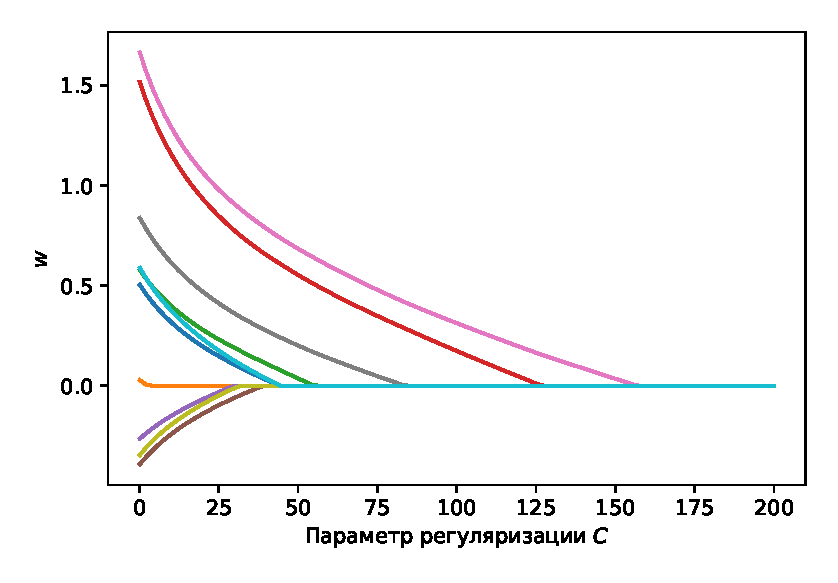
\includegraphics[width=0.5\textwidth]{../figures/log_reg_cs_exp.eps}
	\caption{Sample figure caption.}
	\label{fig:fig1}
\end{figure}

\subsection{Tables}
See awesome Table~\ref{tab:table}.

The documentation for \verb+booktabs+ (`Publication quality tables in LaTeX') is available from:
\begin{center}
	\url{https://www.ctan.org/pkg/booktabs}
\end{center}


\begin{table}
	\caption{Sample table title}
	\centering
	\begin{tabular}{lll}
		\toprule
		\multicolumn{2}{c}{Part}                   \\
		\cmidrule(r){1-2}
		Name     & Description     & Size ($\mu$m) \\
		\midrule
		Dendrite & Input terminal  & $\sim$100     \\
		Axon     & Output terminal & $\sim$10      \\
		Soma     & Cell body       & up to $10^6$  \\
		\bottomrule
	\end{tabular}
	\label{tab:table}
\end{table}

\subsection{Lists}
\begin{itemize}
	\item Lorem ipsum dolor sit amet
	\item consectetur adipiscing elit.
	\item Aliquam dignissim blandit est, in dictum tortor gravida eget. In ac rutrum magna.
\end{itemize}


\bibliographystyle{unsrtnat}
\bibliography{references}

\end{document}